\documentclass[10pt]{beamer}

\usepackage[utf8]{inputenc}
\usepackage{tcolorbox}
\usepackage{tikz}
\usepackage{tikz-3dplot}
\usetikzlibrary{intersections,calc,,angles,quotes,through}
\usepackage{amsmath}
\usepackage{graphicx}
\usepackage{cases}
\def \heart {\textcolor{blue}{$\heartsuit$} }
\def \C {\mathcal{C}}
\def \orthog {\underline{\perp}}
\def\arcos{\operatorname{arcos}}
\def \deg {^{\circ}}

\newcommand{\vect}[1] {
  \overrightarrow{#1}}

\tcbset{%
	basic/.style={colframe=black,
		      colback=white,
		      top= 0mm,
		      bottom = 2mm,
		      boxsep=0mm
		      }
}
\tikzset{
    invisible/.style={opacity=0},
    visible on/.style={alt={#1{}{invisible}}},
    alt/.code args={<#1>#2#3}{%
      \alt<#1>{\pgfkeysalso{#2}}{\pgfkeysalso{#3}} % \pgfkeysalso doesn't change the path
    },
  }

    
\begin{document}  
    \beamertemplatenavigationsymbolsempty
    \setlength{\abovedisplayskip}{0pt}
    \setlength{\belowdisplayskip}{0pt}
    \frame{
	  
	  \frametitle{Q5 Septembre 2003.}
	  \renewcommand{\theenumi}{\alph{enumi})}
	  On considère les droites $d_1$ et $d_2$ données par leurs équations dans un repère
	  orthonormé de l’espace : \\ \medskip
	  $$ d_1 \equiv \begin{cases}
	                 2x - y = 0 \\
	                 3x - z = 0
	                \end{cases},	                
	     d_2 \equiv \begin{cases}
	                 x =1 \\
	                 2y - z = 0
	                \end{cases}.$$
	  \begin{enumerate}
	   \item Montrer que $d_1$ et $d_2$ sont gauches.
	   \item Ecrire l'équation du plan $\pi$ parallèle à $d_1$ et à $d_2$ et qui contient le point $P$ de coordonnées $(1, 1, 1)$.
	   \item Ecrire l’équation d’une droite $d_3$, perpendiculaire à $\pi$ et qui s’appuie sur $d_1$ et $d_2$.
	  \end{enumerate}


	  \vfill
	  
	  \pause
	  
	   \begin{tcolorbox}[basic] \smallskip
	     \centering\underline{Traduction} \smallskip
	     \begin{columns}[c]
	     \column{.333\textwidth}\centering 
	     \renewcommand{\theenumi}{\alph{enumi})}
	     \begin{enumerate}
	      \item $d_1,d_2$ sont :\\ \smallskip ni parallèles, \\ni sécantes. 
	     \end{enumerate}
	     
	     \column{.333\textwidth}\centering 
	     \begin{enumerate}
	      \item[b).] $\pi \equiv\begin{cases}
				     \vect{d_1}, \\[0.2em]
				     \vect{d_2}, \\
				     \ni P.
	                            \end{cases}$
	     \end{enumerate}

	     \column{.333\textwidth}\centering 
	      \begin{enumerate}
	      \item[c).] $d_3 \equiv\begin{cases}
				     \vect{n_\pi}, \\[0.2em]
				     d_3 \nmid d_1, \\
				     d_3 \nmid d_2.
	                            \end{cases}$
	     \end{enumerate}
	  \end{columns}
	  \end{tcolorbox}
    }

    \frame{ 
	  % résolution ex1

		
				  \begin{tcolorbox}[basic] \smallskip
				  \centering\underline{Traduction} \smallskip
				  \begin{columns}[c]
				  \column{.333\textwidth}\centering 
				  \renewcommand{\theenumi}{\alph{enumi})}
				  \begin{enumerate}
				    \item $d_1,d_2$ sont :\\ \smallskip ni parallèles, \\ni sécantes. 
				  \end{enumerate}
				  
				  \column{.333\textwidth}\centering 
				  \begin{enumerate}
				    \item[b).] $\pi \equiv\begin{cases}
							  \vect{d_1}, \\[0.2em]
							  \vect{d_2}, \\
							  \ni P.
							  \end{cases}$
				  \end{enumerate}

				  \column{.333\textwidth}\centering 
				    \begin{enumerate}
				    \item[c).] $d_3 \equiv\begin{cases}
							  \vect{n_\pi}, \\[0.2em]
							  d_3 \nmid d_1, \\
							  d_3 \nmid d_2.
							  \end{cases}$
				  \end{enumerate}
				\end{columns}
				\end{tcolorbox}
		
		
		
		\centering\underline{Résolution}\\ \flushleft
		\begin{columns}[c]
		\column{.5\textwidth}\centering 
		\begin{align*}
		 d_1 &\equiv \begin{cases} 
			     2x - y = 0, \\
			     3x - z = 0.
		             \end{cases}\\
		     &\equiv \begin{cases}
			      \vect{d_1} = (1,2,3), \\
			      D_1 = (0,0,0).
		             \end{cases}     
		\end{align*}		
		
		\column{.5\textwidth}\centering 
		\begin{align*}
		 d_2&\equiv \begin{cases} 
		       x =1, \\
	               2y - z = 0.
		            \end{cases} \\
		    &\equiv \begin{cases}
			    \vect{d_2} = (0,1,2), \\
			    D_2 = (1,1,2).
			    \end{cases}
		\end{align*}
		\end{columns}  \medskip
		$\vect{d_1}$ n'est pas multiple de $\vect{d_2}$ $\qquad \rightarrow \qquad$ $d_1,d_2$ non parallèles. \\ \medskip
		Système $d_1 \cap d_2$ impossible $\qquad \rightarrow \qquad$ $d_1,d_2$ non sécantes. \\ \medskip
		$d_1,d_2$ sont gauches. \hfill $\qed(a)$

    }
	 \frame{ 
	  % résolution ex1

		
				  \begin{tcolorbox}[basic] \smallskip
				  \centering\underline{Traduction} \smallskip
				  \begin{columns}[c]
				  \column{.333\textwidth}\centering 
				  \renewcommand{\theenumi}{\alph{enumi})}
				  \begin{enumerate}
				    \item $d_1,d_2$ sont :\\ \smallskip ni parallèles, \\ni sécantes. 
				  \end{enumerate}
				  
				  \column{.333\textwidth}\centering 
				  \begin{enumerate}
				    \item[b).] $\pi \equiv\begin{cases}
							  \vect{d_1}, \\[0.2em]
							  \vect{d_2}, \\
							  \ni P.
							  \end{cases}$
				  \end{enumerate}

				  \column{.333\textwidth}\centering 
				    \begin{enumerate}
				    \item[c).] $d_3 \equiv\begin{cases}
							  \vect{n_\pi}, \\[0.2em]
							  d_3 \nmid d_1, \\
							  d_3 \nmid d_2.
							  \end{cases}$
				  \end{enumerate}
				\end{columns}
				\end{tcolorbox}
		
		
		
		\bigskip
		\begin{columns}[c]
		\column{.5\textwidth}\centering 
		
		 $d_1 \equiv \begin{cases}
			      \vect{d_1} = (1,2,3), \\
			      D_1 = (0,0,0).
		             \end{cases}$     
				
		
		\column{.5\textwidth}\centering 
		
		 $d_2  \equiv \begin{cases}
			      \vect{d_2} = (0,1,2), \\
			      D_2 = (1,1,2).
			      \end{cases}$
		\end{columns}  
		\bigskip\centering
		$\pi \equiv\begin{cases}
			   \vect{d_1}, \\[0.2em]
			   \vect{d_2}, \\
			   \ni P(1,1,1).
			   \end{cases} \qquad \rightarrow \qquad \pi \equiv x-2y+z=0.$ \\
			   \hfill $\qed(b)$

    }  
  
  
  \frame{ \onslide<+->
	  % résolution ex1

		
				  \begin{tcolorbox}[basic] \smallskip
				  \centering\underline{Traduction} \smallskip
				  \begin{columns}[c]
				  \column{.333\textwidth}\centering 
				  \renewcommand{\theenumi}{\alph{enumi})}
				  \begin{enumerate}
				    \item $d_1,d_2$ sont :\\ \smallskip ni parallèles, \\ni sécantes. 
				  \end{enumerate}
				  
				  \column{.333\textwidth}\centering 
				  \begin{enumerate}
				    \item[b).] $\pi \equiv\begin{cases}
							  \vect{d_1}, \\[0.2em]
							  \vect{d_2}, \\
							  \ni P.
							  \end{cases}$
				  \end{enumerate}

				  \column{.333\textwidth}\centering 
				    \begin{enumerate}
				    \item[c).] $d_3 \equiv\begin{cases}
							  \vect{n_\pi}, \\[0.2em]
							  d_3 \nmid d_1, \\
							  d_3 \nmid d_2.
							  \end{cases}$
				  \end{enumerate}
				\end{columns}
				\end{tcolorbox}
		
		
		
		
		\begin{columns}[c]
		\column{.5\textwidth}\centering 
		
		 $d_1 \equiv \begin{cases}
			      \vect{d_1} = (1,2,3), \\
			      D_1 = (0,0,0).
		             \end{cases}$     
				
		
		\column{.5\textwidth}\centering 
		
		 $d_2  \equiv \begin{cases}
			      \vect{d_2} = (0,1,2), \\
			      D_2 = (1,1,2).
			      \end{cases}$
		\end{columns}  
		\vspace{-3mm}
		\begin{columns}
		\column{.5\textwidth}\flushleft
		\heart Une droite de direction $\vect{n_\pi}$ et d'appui sur deux droites $d_1$ et $d_2$,
		est l'intersection du plan contenant $d_1$ et la direction $\vect{n_\pi}$ avec le plan contenant $d_2$ et la direction $\vect{n_\pi}$.
		\column{.5\textwidth}\centering 
				  \begin{figure}[h]
				  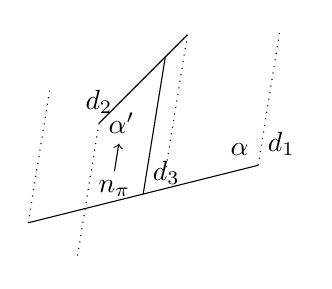
\begin{tikzpicture}[scale=0.73]
			          %projection ($(X)!(B')!(B)$)
			          %nommer chemin 'name path
			          %intersection \path [name intersections={of=d and gb,by=G}];
			          
			          %\draw[help lines] (-3,-3) grid (3,3);
			          \draw (-2,-0.5,0) -- (2,0.5,0) node[above right] {$d_1$};
			          \draw (0,2,-2) -- (0,2,2) node[above] {$d_2$};
			          \draw[visible on =<5>]  (0,0,0)  node[above right] {$d_3$} -- (0,2,-1);
			          
			          \draw[visible on=<2-4>,->,xshift=-5mm,yshift=-6mm] (0,1,0) node[below] {$n_\pi$} -- +(0,0.4,-0.2); 
			          
			          \draw[dotted,visible on=<{3,5}>] (-2,-0.5,0) -- +(0,2,-1) (2,0.5,0) node[above left]{$\alpha$} -- +(0,2,-1);
			          \draw[dotted,visible on=<4-5>] (0,2,2)  node[right]{$\alpha '$} -- +(0,-2,1) (0,2,-2) -- +(0,-2,1);
				  \end{tikzpicture}
				  \end{figure}
		\end{columns}
		
		\vspace{-2mm}
		\onslide<+->
		$\pi \equiv x-2y+z=0. \rightarrow \vect{n_\pi}=(1,-2,1)$. \\
		
		\vspace{-6mm}
		
		
		\begin{columns}[c]

		\column{.333\textwidth}\flushleft 
		\onslide<+->
		\begin{align*}
		\alpha \equiv& \begin{cases}
		                D_1, \\
		                \vect{d_1}, \\
		                \vect{n_\pi}.
		               \end{cases} \\
		       \equiv&\ 4x+y-2z=0.
		\end{align*}
		
		\column{.333\textwidth}\flushleft 
		\onslide<+->
		\begin{align*}
		\alpha' \equiv& \begin{cases}
		                D_2, \\
		                \vect{d_2}, \\
		                \vect{n_\pi}.
		               \end{cases} \\
		       \equiv&\ 5x +2y -z -5=0.
		\end{align*}
		
		\column{.333\textwidth}\flushleft 
		\onslide<+->
		\begin{align*}
		 d_3      =&\ \alpha \cap \alpha ', \\
		     \equiv&\ x-\frac{5}{6} = \dfrac{y-\frac{5}{3}}{-2} = z - \frac{5}{2}.
		\end{align*}
		\hfill $\qed(c)$\hspace{-3mm}
		\vspace{-3mm}
		\end{columns}

		

    } 
\end{document}
